\tikzstyle{lien} = [->, >=latex]
\tikzstyle{basic_text}=[text width=2cm, text badly centered]
\tikzstyle{basic_node}=[draw = black,rounded corners=4pt, basic_text]
\tikzstyle{wrapper}=[basic_node, inner sep=3pt]
\tikzstyle{hidden}=[draw=black!0,color=black!0]
\tikzstyle{faded}=[draw=black!20, color=black!20]

\newcounter{i}
\forloop{i}{0}{\value{i} < 10}{
    \ifcase\arabic{i}
      {}
      \or
      \section{Analyse lexicale}

\begin{frame}
  \frametitle{Principe général de l'analyse lexicale}
  \begin{tikzpicture}
    \node (0, 0) {}; % to align the scope
    \begin{scope} [shift={(5.5, 0)}]
      \node [basic_node, text width=4.5cm, align=left] (Fortran){
      \scalebox{0.8}{
        \parbox{\textwidth}{
          \textbf{Programme Fortran}
          \inputminted[firstline=1, lastline=3, linenos=false]{fortran}{static/HelloWorld.f90}
        }
      }
    };

    \node [basic_node, text width=10.5cm, align=left, below=1cm of Fortran] (C) {
      \scalebox{0.8}{
        \parbox{\textwidth}{
          \textbf{Liste de lexèmes}
          \footnotesize\inputminted[frame=none, xleftmargin=0pt, linenos=false, breaklines=false]{ocaml}{static/listeLexemes.ml}
        }
      } 
    };

    \draw [lien, thick] (Fortran.south) to (C.north);
    \end{scope}
  \end{tikzpicture}
\end{frame}

%----------------regex----------------
\subsection{Les expressions régulières}
\tikzstyle{box}=[draw, rounded corners=4pt]
\tikzstyle{frame}=[box, minimum width=11.3cm, minimum height=6cm]
\tikzstyle{faded}=[color=black!25]
\tikzstyle{hidden}=[draw=white!0, color=white!0]

\begin{frame}
  \frametitle{Les expressions régulières\esp}
  \begin{tikzpicture}
    % frame
    \node[frame] (frame) {};

    \node[below=0.5cm of frame.north west, anchor=north west] (1) {\point Expressions régulières};
    \node[faded, below=0.6cm of 1.west, anchor=west] {\point Automates};
    
    \node[below=4cm of frame.west, anchor=west, box] (state_1) {\scriptsize Analyse lexicale};
    \node[right=0.5cm of state_1.east, anchor=west, box, faded] (state_2) {\scriptsize Analyse syntaxique};
    \node[right=0.5cm of state_2.east, anchor=west, box, faded] (state_3) {\scriptsize Abstraction};
    \node[right=0.5cm of state_3.east, anchor=west, box, faded] (state_4) {\scriptsize Conversion};
    \draw[->, >=latex, faded] (state_1.east) -- (state_2.west);
    \draw[->, >=latex, faded] (state_2.east) -- (state_3.west);
    \draw[->, >=latex, faded] (state_3.east) -- (state_4.west);
    \draw[dashed] (frame.south west) -- (state_1.north west);
    \draw[dashed] (frame.south east) -- (state_1.north east);

    % definition
    \only<1->{
      \node[right=1.5 cm of 1] (def) {définies inductivement sur:};
      \node[below] at (def.south) (_1) {$\emptyset,\,\varepsilon,\, a \in\Sigma$};
    }
    \only<2->{
      \node[below=0.35cm] at (_1.south) (_2) {avec les règles usuelles:};
      \node[below] at (_2.south) (_3) {$\cdot,\ |,\ *$ };
    }
    \only<3->{
      \node[below=0.35cm] at (_3.south) (_4) {et des additionnelles:};
      \node[below] at (_4.south) {$+,\ ?,\ [a-z],\ \sim$};
    }

    % exemple
    \only<4->{
      \node[below=1.6cm of 1.south] (exmpl) {$\ \ $exemple:};
      \node[below, anchor=north east] (part0) at (exmpl.south) {[0 - 9]$^+$}; \node[right = -4pt] (part1) at (part0.east) {$\cdot$}; \node[right=-4pt] (part2) at (part1.east) {(,[0 - 9]$^+$)?};
    }
    \node<5->[fit=(part0), draw=blue, rounded corners=4pt, inner sep=-1.5pt]{};
    \node<6->[fit=(part2), draw=red, rounded corners=4pt, inner sep=-1.5pt]{};
    \only<7->{
      \node[below=1cm of part0.west, anchor=west] (part10) {"};
      \node[right = -4pt] (part11) at (part10.east) {$\cdot$};
      \node[right = -4pt] (part12) at (part11.east) {($\sim$")$^*$};
      \node[right = -4pt] (part13) at (part12.east) {$\cdot$};
      \node[right = -4pt] (part14) at (part13.east) {"};
    }
    \node<8->[fit=(part10), draw=vertFonce, rounded corners=4pt, inner sep=-1.5pt]{};
    \node<8->[fit=(part14), draw=vertFonce, rounded corners=4pt, inner sep=-1.5pt]{};
    \node<9->[fit=(part12), draw=violet, rounded corners=4pt, inner sep=-1.5pt]{};
  \end{tikzpicture}
\end{frame}

%---------------automates--------------
\subsection{Les automates}
\begin{frame}
  \frametitle{Les automates\esp}
  \begin{tikzpicture}
    % frame
    \node[frame] (frame) {};

    \node[below=0.5cm of frame.north west, anchor=north west, faded] (1) {\point Expressions régulières};
    \node[below=0.6cm of 1.west, anchor=west] (_2) {\point Automates};

    \node[below=4cm of frame.west, anchor=west, box] (state_1) {\scriptsize Analyse lexicale};
    \node[right=0.5cm of state_1.east, anchor=west, box, faded] (state_2) {\scriptsize Analyse syntaxique};
    \node[right=0.5cm of state_2.east, anchor=west, box, faded] (state_3) {\scriptsize Abstraction};
    \node[right=0.5cm of state_3.east, anchor=west, box, faded] (state_4) {\scriptsize Conversion};
    \draw[->, >=latex, faded] (state_1.east) -- (state_2.west);
    \draw[->, >=latex, faded] (state_2.east) -- (state_3.west);
    \draw[->, >=latex, faded] (state_3.east) -- (state_4.west);
    \draw[dashed] (frame.south west) -- (state_1.north west);
    \draw[dashed] (frame.south east) -- (state_1.north east);

    % definition
    \only<1->{\node[right=4.5 cm of _2] (def) {$\mathcal{A}=(\Sigma, Q, I, F, \delta)$};}
    \only<2->{
      \begin{scope}
        [below=1.5cm of def.south, scale=0.8, every node/.style={scale=0.8}, initial text=, shift={(0.8, 0)}]

        \node [state, initial]         (1) at (0, 0)        {1};
        \node [state]                  (2) [right=1cm of 1] {2};
        \node [state, accepting right] (3) [right=1cm of 2] {3};

        \path[->]
        (1) edge              node [above] {$a$} (2)
        (2) edge              node [above] {$c$} (3)
        (2) edge [loop above] node [above] {$b$} (2)
        ;
      \end{scope}
      \node [below=2.2cm of def.south, font=\scriptsize] {Automate qui a pour langage $a\cdot b^*\cdot c$};
    }
  \end{tikzpicture}
\end{frame}

%------------étude d'un exemple-----------
\begin{frame}
  \frametitle{Les automates: étude d'un exemple\esp}
  \begin{tikzpicture}
    \node at (3, 0) (text) {\ttfamily print*,"Hello World"};
    \begin{scope}
      [every node/.style={scale=0.6,font=\Large}, scale=0.4, initial text=, shift={(-13, 0)}]
      \tikzstyle{style0}=[]
      \tikzstyle{style1}=[]
      \tikzstyle{style2}=[]
      \tikzstyle{style3}=[]
      \tikzstyle{style4}=[] 
      \tikzstyle{style5}=[]
      \tikzstyle{style6}=[]
      \tikzstyle{style7}=[]
      \tikzstyle{style8}=[]
      \tikzstyle{style9}=[]

      \only<1> {\tikzstyle{style0}=[draw=blue!50,very thick,fill=blue!20]}
      \only<2> {\tikzstyle{style1}=[draw=blue!50,very thick,fill=blue!20]}
      \only<3> {\tikzstyle{style2}=[draw=blue!50,very thick,fill=blue!20]}
      \only<4> {\tikzstyle{style3}=[draw=blue!50,very thick,fill=blue!20]}
      \only<5> {\tikzstyle{style4}=[draw=blue!50,very thick,fill=blue!20]}
      \only<6> {\tikzstyle{style5}=[draw=blue!50,very thick,fill=blue!20]}
      \only<7> {\tikzstyle{style0}=[draw=blue!50,very thick,fill=blue!20]}
      \only<8> {\tikzstyle{style8}=[draw=blue!50,very thick,fill=blue!20]}
      \only<9> {\tikzstyle{style0}=[draw=blue!50,very thick,fill=blue!20]}
      \only<10>{\tikzstyle{style9}=[draw=blue!50,very thick,fill=blue!20]}
      \only<11> {\tikzstyle{style0}=[draw=blue!50,very thick,fill=blue!20]}
      \only<12-23>{\tikzstyle{style6}=[draw=blue!50,very thick,fill=blue!20]}
      \only<24>{\tikzstyle{style7}=[draw=blue!50,very thick,fill=blue!20]}

      \node[state, style0, initial        ]  at (0,0) (0)          {$I$};

      \node[state, style1] (1) at (2,1) {1};
      \node[state, style2] (2) [right=0.4cm of 1] {2};
      \node[state, style3] (3) [right=0.4cm of 2] {3};
      \node[state, style4] (4) [right=0.4cm of 3] {4};
      \node[state, accepting right, style5] (5) [right=0.4cm of 4] {$F_1$};
      
      \node[state, style6,                ] (6) at (2,3) {5};
      \node[state, style7, accepting right] (7) [right=0.4cm of 6] {$F_2$};
      
      \node[state, style8, accepting right] (8) at (2,-1)      {$F_3$};
      \node[state, style9, accepting right] (9) at (2,-3)      {$F_4$};

      \path[->]
      (0) edge                node[above] {$*$} (8)
      (0) edge                node[above] {\LARGE$,$} (9)

      (0) edge                node[above] {$p$} (1)
      (1) edge                node[above] {$r$} (2)
      (2) edge                node[above] {$i$} (3)
      (3) edge                node[above] {$n$} (4)
      (4) edge                node[above] {$t$} (5)
      
      
      (0) edge                node[above] {$"$} (6)
      (6) edge [loop above]   node[above] {$\sim"$} (6)
      (6) edge                node[above] {$"$} (7)
      ;
      
    \end{scope}
    \foreach \step in {1,2,...,6}{
      \node<\step>[right=\fpeval{\step * 5.75 - 3}pt of text.west, draw=blue, fill=blue!20, inner sep=0pt, minimum width=2pt, minimum height=10pt]{};
    }
    \foreach \step in {7,8}{
      \node<\step>[right=\fpeval{(\step - 1) * 5.75 - 3}pt of text.west, draw=blue, fill=blue!20, inner sep=0pt, minimum width=2pt, minimum height=10pt]{};
    }
    \foreach \step in {9,10}{
      \node<\step>[right=\fpeval{(\step - 2) * 5.75 - 3}pt of text.west, draw=blue, fill=blue!20, inner sep=0pt, minimum width=2pt, minimum height=10pt]{};
    }
    \foreach \step in {11,12,...,24}{
      \node<\step>[right=\fpeval{(\step - 3) * 5.75 - 3}pt of text.west, draw=blue, fill=blue!20, inner sep=0pt, minimum width=2pt, minimum height=10pt]{};
    }

    \node at (0, -2.3) (lb) {
      \begin{minipage}{\textwidth}
        \only<1-6>  {\inputminted[firstline=1, lastline=1, linenos=false, frame=none, xleftmargin=0pt,]{ocaml}{static/exampleList.ml}}
        \only<7-8>  {\inputminted[firstline=2, lastline=2, linenos=false, frame=none, xleftmargin=0pt,]{ocaml}{static/exampleList.ml}}
        \only<9-10> {\inputminted[firstline=3, lastline=3, linenos=false, frame=none, xleftmargin=0pt,]{ocaml}{static/exampleList.ml}}
        \only<11-24>{\inputminted[firstline=4, lastline=4, linenos=false, frame=none, xleftmargin=0pt,]{ocaml}{static/exampleList.ml}}
        \only<25>   {\inputminted[firstline=5, lastline=5, linenos=false, frame=none, xleftmargin=0pt,]{ocaml}{static/exampleList.ml}}
      \end{minipage}
    };
  \end{tikzpicture}
\end{frame}

%------------étude d'un exemple 2-----------
\begin{frame}
  \frametitle{Les automates: étude d'un exemple\esp}
  \begin{tikzpicture}
    \node at (1, 0) (text1) {\ttfamily print};
    \node [right=-5pt of text1.east, anchor=west] (text2) {\ttfamily print};
    \node [right=-5pt of text2.east, anchor=west] (text3) {\ttfamily "Hello World"};

    \begin{scope}
      [every node/.style={scale=0.6,font=\Large}, scale=0.4, initial text=, shift={(-13, 0)}]
      \tikzstyle{style0}=[]
      \tikzstyle{style1}=[]
      \tikzstyle{style2}=[]

      \only<1> {\tikzstyle{style0}=[draw=blue!50,very thick,fill=blue!20]}
      \only<2-3>{\tikzstyle{style1}=[draw=blue!50,very thick,fill=blue!20]}
      \only<4> {\tikzstyle{style2}=[draw=blue!50,very thick,fill=blue!20]}

      \node[state, style0, style1, style2, initial]  at (0,0) (0)          {$I$};

      \node[state, style1] (1) at (2,1) {1};
      \node[state, style1] (2) [right=0.4cm of 1] {2};
      \node[state, style1] (3) [right=0.4cm of 2] {3};
      \node[state, style1] (4) [right=0.4cm of 3] {4};
      \node[state, accepting right, style1] (5) [right=0.4cm of 4] {$F_1$};
      
      \node[state, style2,                ] (6) at (2,3) {5};
      \node[state, style2, accepting right] (7) [right=0.4cm of 6] {$F_2$};
      
      \node[state, accepting right]         (8) at (2,-1)      {$F_3$};
      \node[state, accepting right]         (9) at (2,-3)      {$F_4$};

      \path[->]
      (0) edge                      node[above] {$*$} (8)
      (0) edge                      node[above] {\LARGE$,$} (9)

      (0) edge [style1]             node[above] {$p$} (1)
      (1) edge [style1]             node[above] {$r$} (2)
      (2) edge [style1]             node[above] {$i$} (3)
      (3) edge [style1]             node[above] {$n$} (4)
      (4) edge [style1]             node[above] {$t$} (5)
      
      
      (0) edge [style2]             node[above] {$"$} (6)
      (6) edge [loop above, style2] node[above] {$\sim"$} (6)
      (6) edge [style2]             node[above] {$"$} (7)
      ;
      
    \end{scope}
    
    \node<2>[fit=(text1), draw=blue, fill=blue!20, inner sep=-2pt, fill opacity=0.5]{};
    \node<3>[fit=(text2), draw=blue, fill=blue!20, inner sep=-2pt, fill opacity=0.5]{};
    \node<4>[fit=(text3), draw=blue, fill=blue!20, inner sep=-2pt, fill opacity=0.5]{};
    \node at (0, -2.3) {
      \begin{minipage}{\textwidth}
        \only<1>{\inputminted[firstline=1, lastline=1, linenos=false, frame=none, xleftmargin=0pt,]{ocaml}{static/exampleList.ml}}
        \only<2>{\inputminted[firstline=2, lastline=2, linenos=false, frame=none, xleftmargin=0pt,]{ocaml}{static/exampleList.ml}}
        \only<3>{\inputminted[firstline=6, lastline=6, linenos=false, frame=none, xleftmargin=0pt,]{ocaml}{static/exampleList.ml}}
        \only<4>{\inputminted[firstline=7, lastline=7, linenos=false, frame=none, xleftmargin=0pt,]{ocaml}{static/exampleList.ml}}
      \end{minipage}
    };
  \end{tikzpicture}
\end{frame}

%------------déterminisation-----------
\addtocounter{framenumber}{-1}
\subsection{La déterminisation}
\begin{frame}
  \addtocounter{framenumber}{1}
  \frametitle{La déterminisation\esp}

  \begin{tikzpicture}
    % frame
    \begin{scope}
      \node[frame] (frame) {};
      
      \node[below=4cm of frame.west, anchor=west, box] (state_1) {\scriptsize Analyse lexicale};
      \node[right=0.5cm of state_1.east, anchor=west, box, faded] (state_2) {\scriptsize Analyse syntaxique};
      \node[right=0.5cm of state_2.east, anchor=west, box, faded] (state_3) {\scriptsize Abstraction};
      \node[right=0.5cm of state_3.east, anchor=west, box, faded] (state_4) {\scriptsize Conversion};
      \draw[->, >=latex, faded] (state_1.east) -- (state_2.west);
      \draw[->, >=latex, faded] (state_2.east) -- (state_3.west);
      \draw[->, >=latex, faded] (state_3.east) -- (state_4.west);
      \draw[dashed] (frame.south west) -- (state_1.north west);
      \draw[dashed] (frame.south east) -- (state_1.north east);
    \end{scope}

    % automatons
    \only<1,2>{
      \begin{scope}[initial text=, scale=0.9, shift={(-5, 0)}]
        \node[state, initial] (0) at (0, 0) {0};
        \node[state] (1) at (1.3, 1) {1};
        \node[state] (2) at (1.3, -1) {2};
        \node[state, right=0.5cm of 1, accepting right] (3) {3};
        \node[state, right=0.5cm of 2, accepting right] (4) {4};

        \path[->]
        (0) edge node[above] {$a$} (1)
        (0) edge node[above] {$a$} (2)
        (1) edge node[above] {$b$} (3)
        (2) edge node[above] {$c$} (4)
        ;
      
      \end{scope}
    }
      
    \only<1,3>{
      \begin{scope}[shift={(1.4, 0)}, initial text=, scale=0.9]
        \node[state, initial] (0) at (0, 0) {0};
        \node[state, right=0.5cm of 0] (1) {\{1,2\}};
        \node[state, accepting right] (3) at (3.3, 1) {3};
        \node[state, accepting right] (4) at (3.3, -1) {4};

        \path[->]
        (0) edge node[above] {$a$} (1)
        (1) edge node[above] {$b$} (3)
        (1) edge node[above] {$c$} (4)
        ;
      \end{scope}
    }

    \node<1> at (0, -2.7) {\footnotesize Deux automates reconnaisants $(ab)|(ac)$};

    \only<2>{
      \begin{scope}[shift={(2.5, 0)}]
        \node{
          \begin{minipage}{0.55\textwidth}
            \inputminted[firstline=7, lastline=12,firstnumber=1]{ocaml}{../../src/automates.ml}
          \end{minipage}
        };
      \end{scope}
    }

    \only<3>{
      \begin{scope}[shift={(-2.5, 0)}]
        \node{
          \begin{minipage}{0.55\textwidth}
            \inputminted[firstline=29, lastline=34,firstnumber=1]{ocaml}{../../src/automates.ml}
          \end{minipage}
        };
      \end{scope}
    }
  \end{tikzpicture}
\end{frame}
      \or
      \section{Analyse syntaxique}
\begin{frame}
  \frametitle{Principe général de l'analyse syntaxique}
  \begin{tikzpicture}
    \node (0, 0) {}; % to align the scope
    \begin{scope} [shift={(5.5, 0)}]
      \node [basic_node, text width=10.5cm, align=left] (Fortran) {
        \scalebox{0.8}{
          \parbox{\textwidth}{
            \textbf{Liste de lexèmes}
            \footnotesize \inputminted[frame=none, xleftmargin=0pt, linenos=false, breaklines=false]{ocaml}{static/listeLexemes.ml}
          }
        } 
      };

      \node [basic_node, text width=10cm, below=1cm of Fortran, align=left] (C) {
        \scalebox{0.8}{\textbf{Arbre de syntaxe}}
        \scalebox{0.85}{\tikzstyle{feuille}=[draw, rectangle, inner sep = 0.12cm]
\tikzstyle{noeud}=[draw, rectangle,rounded corners, minimum width= 0.64cm, line width = 1pt]
\begin{tikzpicture}[
        baseline=(base), 
        level/.style={sibling distance = 2cm/#1, level distance = 1cm},
        every node/.style={scale=0.6, font=\footnotesize}
    ]
    
    \node[ noeud] {Programme}
    child { 
        node[ noeud] (base) {ProgramMC}
        child { 
            node [ feuille] {program}
        }
    }
    child { 
        node[ noeud] {NLigne}
        child { 
            node [ feuille] {\textbackslash n}
        }
    }
    child [ level distance=2cm]{ 
        node [ noeud] {Print}
        child {
            node [noeud] {PrintMC}
            child { 
                node [ feuille] {print}
            }
        }
        child{
            node [noeud] {Asterisque}
            child { 
                node [feuille] {*}
            }
        }
        child{
            node [noeud] {Virgule}
            child { 
                node [feuille] {,}
            }
        }
        child{
            node [noeud] {Chaine}
            child { 
                node [feuille] {"Hello World"}
            }
        }
        child{
            node [noeud] {Paramliste}
            child { 
                node [feuille] {$\varepsilon$}
            }
        }
    }
    child { 
        node[ noeud] {EndProgramMC}
        child { 
            node [ feuille] {end program}
        }
    };

\end{tikzpicture}}
      };

      \draw [lien, thick] (Fortran.south) to (C.north);
    \end{scope}
  \end{tikzpicture}
\end{frame}

\tikzstyle{box}=[draw, rounded corners=4pt]
\tikzstyle{frame}=[box, minimum width=11.3cm, minimum height=6cm]
\tikzstyle{faded}=[color=black!25]
\tikzstyle{hidden}=[draw=white!0, color=white!0]

%------------grammaire-----------
\subsection{La grammaire}
\begin{frame}
  \frametitle{Analyse syntaxique\esp}

  \begin{tikzpicture}
    % frame
    \node[frame] (frame) {};

    \node[below=0.5cm of frame.north west, anchor=north west] (1) {\point Grammaire};
    \node[faded, below=0.6cm of 1.west, anchor=west] (_2) {\point LL1};

    \tikzstyle{faded}=[draw=black!20,color=black!20]
    \node[below=4cm of frame.west, anchor=west, box, faded] (state_1) {\scriptsize Analyse lexicale};
    \node[right=0.5cm of state_1.east, anchor=west, box] (state_2) {\scriptsize Analyse syntaxique};
    \node[right=0.5cm of state_2.east, anchor=west, box, faded] (state_3) {\scriptsize Abstraction};
    \node[right=0.5cm of state_3.east, anchor=west, box, faded] (state_4) {\scriptsize Conversion};
    \draw[->, >=latex, faded] (state_1.east) -- (state_2.west);
    \draw[->, >=latex, faded] (state_2.east) -- (state_3.west);
    \draw[->, >=latex, faded] (state_3.east) -- (state_4.west);
    \draw[dashed] (frame.south west) -- (state_2.north west);
    \draw[dashed] (frame.south east) -- (state_2.north east);

    % définition 
    \only<1->{
      \node[right=4.2cm of 1.east, anchor=west] (def) {$\mathcal{G}=(\Sigma, V, P, \mathcal{S})$};
      \node[below=0.25cm, font=\ttfamily] (def1) at (def) {$R\in V\rightarrow W_1...W_n \in (V\times\Sigma)^{n}$};
    }

    % exemple simple
    \only<2->{
      \node[below=0.2 cm of def1] {Exemple:};
      \node[below=1.4cm of def.200, anchor = north west] {
        \begin{minipage}{0.5\textwidth}
          \inputminted[linenos=true]{text}{static/Grammaire_example.txt}
        \end{minipage}
      };
      \node[below=4.4cm of def.200, font=\scriptsize, anchor=west] {Grammaire de $a^* \cdot b^*$};
    }

    % application à une chaine simple
    \only<3->{
      \begin{scope}[shift={(-2.5, 1.8)}, font=\footnotesize]
        \tikzstyle{style1}=[hidden]
        \tikzstyle{style2}=[hidden]
        \tikzstyle{style3}=[hidden]
        \tikzstyle{style4}=[hidden]
        \tikzstyle{style5}=[hidden]

        \only<4->{\tikzstyle{style1}=[font=\ttfamily]}
        \only<5->{\tikzstyle{style2}=[font=\ttfamily]}
        \only<6->{\tikzstyle{style3}=[font=\ttfamily]}
        \only<7->{\tikzstyle{style4}=[font=\ttfamily]}
        \only<8->{\tikzstyle{style5}=[font=\ttfamily]}

        \node [font=\ttfamily] (0) at (0, 0) {S};
        \node [below=0.3cm of 0, style1] (1) {A};
        \node [below=0.3cm of 1.south west, style2] (2) {$a$};
        \node [below=0.3cm of 1.south east, style2] (3) {A};
        \node [below=0.3cm of 3, style3] (4) {B};
        \node [below=0.3cm of 4.south west, style4] (5) {$b$};
        \node [below=0.3cm of 4.south east, style4] (6) {B};
        \node [below=0.3cm of 6, style5] (7) {$\varepsilon$};

        \draw [style1] (0) -- (1);
        \draw [style2] (1) -- (2);
        \draw [style2] (1) -- (3);
        \draw [style3] (3) -- (4);
        \draw [style4] (4) -- (5);
        \draw [style4] (4) -- (6);
        \draw [style5] (6) -- (7);
      \end{scope}
    }

  \end{tikzpicture}

\end{frame}

%-------------LL1--------------
\subsection{L'algorithme LL1}
\begin{frame}
  \begin{tikzpicture}
    % frame
    \node[frame] (frame) {};

    \node[below=0.5cm of frame.north west, anchor=north west, faded] (1) {\point Grammaire};
    \node[below=0.6cm of 1.west, anchor=west] (_2) {\point LL1};

    \tikzstyle{faded}=[draw=black!20,color=black!20]
    \node[below=4cm of frame.west, anchor=west, box, faded] (state_1) {\scriptsize Analyse lexicale};
    \node[right=0.5cm of state_1.east, anchor=west, box] (state_2) {\scriptsize Analyse syntaxique};
    \node[right=0.5cm of state_2.east, anchor=west, box, faded] (state_3) {\scriptsize Abstraction};
    \node[right=0.5cm of state_3.east, anchor=west, box, faded] (state_4) {\scriptsize Conversion};
    \draw[->, >=latex, faded] (state_1.east) -- (state_2.west);
    \draw[->, >=latex, faded] (state_2.east) -- (state_3.west);
    \draw[->, >=latex, faded] (state_3.east) -- (state_4.west);
    \draw[dashed] (frame.south west) -- (state_2.north west);
    \draw[dashed] (frame.south east) -- (state_2.north east);

    % petite description de LL1
    \node[font=\ttfamily] (list) at (-4, 0){[a, b]};
    \node[right] (+) at (list.east) {et};
    \node[right] at (+.east) {
        \begin{minipage}{0.5\textwidth}
          \inputminted{text}{static/Grammaire_example.txt}
        \end{minipage}
    };
    \only<2>{
      \node[font=\ttfamily] at (0.5, 0) {$\Rightarrow$};
      \begin{scope}[shift={(2.5, 1.8)}, font=\footnotesize]
        
        \node [font=\ttfamily] (0) at (0, 0) {S};
        \node [below=0.3cm of 0, font=\ttfamily] (1) {A};
        \node [below=0.3cm of 1.south west, font=\ttfamily] (2) {$a$};
        \node [below=0.3cm of 1.south east, font=\ttfamily] (3) {A};
        \node [below=0.3cm of 3, font=\ttfamily] (4) {B};
        \node [below=0.3cm of 4.south west, font=\ttfamily] (5) {$b$};
        \node [below=0.3cm of 4.south east, font=\ttfamily] (6) {B};
        \node [below=0.3cm of 6] (7) {$\varepsilon$};

        \draw (0) -- (1);
        \draw (1) -- (2);
        \draw (1) -- (3);
        \draw (3) -- (4);
        \draw (4) -- (5);
        \draw (4) -- (6);
        \draw (6) -- (7);
      \end{scope}
    }
    
  \end{tikzpicture}

\end{frame}
      \or
      \section{Conversion vers la syntaxe abstraite}

% TODO ajouter ici une diapo pour expliquer le but général (arbre donné trop gros + pas adapté pour les autres langages que fortran, on le transforme en un arbre de syntaxe abstraite)

\begin{frame}
  \frametitle{Principe général de l'abstraction}
  \begin{tikzpicture}
    \node (0, 0) {}; % to align the scope
    \begin{scope} [shift={(5.5, 0)}]
      \node [basic_node, text width=7cm, align=left] (Fortran) {
        \scalebox{0.8}{\textbf{Arbre de syntaxe}} 
        \scalebox{0.6}{\tikzstyle{feuille}=[draw, rectangle, inner sep = 0.12cm]
\tikzstyle{noeud}=[draw, rectangle,rounded corners, minimum width= 0.64cm, line width = 1pt]
\begin{tikzpicture}[
        baseline=(base), 
        level/.style={sibling distance = 2cm/#1, level distance = 1cm},
        every node/.style={scale=0.6, font=\footnotesize}
    ]
    
    \node[ noeud] {Programme}
    child { 
        node[ noeud] (base) {ProgramMC}
        child { 
            node [ feuille] {program}
        }
    }
    child { 
        node[ noeud] {NLigne}
        child { 
            node [ feuille] {\textbackslash n}
        }
    }
    child [ level distance=2cm]{ 
        node [ noeud] {Print}
        child {
            node [noeud] {PrintMC}
            child { 
                node [ feuille] {print}
            }
        }
        child{
            node [noeud] {Asterisque}
            child { 
                node [feuille] {*}
            }
        }
        child{
            node [noeud] {Virgule}
            child { 
                node [feuille] {,}
            }
        }
        child{
            node [noeud] {Chaine}
            child { 
                node [feuille] {"Hello World"}
            }
        }
        child{
            node [noeud] {Paramliste}
            child { 
                node [feuille] {$\varepsilon$}
            }
        }
    }
    child { 
        node[ noeud] {EndProgramMC}
        child { 
            node [ feuille] {end program}
        }
    };

\end{tikzpicture}}
      };

      \node [basic_node, text width=5.5cm, below=1cm of Fortran, align=left] (C) {
        \scalebox{0.8}{\textbf{Arbre de syntaxe abstraite}}
        \scalebox{0.9}{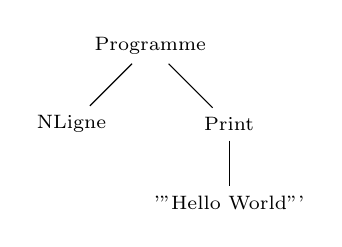
\begin{tikzpicture}

    \node[font=\scriptsize] (0) at (0, 0) {Programme};
    \node[font=\scriptsize] (1) at (-1, -1) {NLigne};
    \node[font=\scriptsize] (2) at (1, -1) {Print};
    \node[font=\scriptsize] (3) at (1, -2) {'"Hello World"'};
    
    \draw (0) -- (1);
    \draw (0) -- (2);
    \draw (2) -- (3);
\end{tikzpicture}}
      };

      \draw [lien, thick] (Fortran.south) to (C.north);
    \end{scope}
  \end{tikzpicture}
\end{frame}

\newcommand{\drawcross}[1]{
  \draw[cross] (#1.north west) -- (#1.south east);
  \draw[cross] (#1.north east) -- (#1.south west);
}

\tikzstyle{cross}=[red, very thick]

%--------------expilaction---------------
\subsection{Fonctionnement}
\begin{frame}
  \frametitle{Syntaxe abstraite\esp}

  \begin{tikzpicture}
    % frame
    \node[frame] (frame) {};
    \tikzstyle{faded}=[draw=black!20,color=black!20]
    
    \node[below=4cm of frame.west, anchor=west, box, faded] (state_1) {\scriptsize Analyse lexicale};
    \node[right=0.5cm of state_1.east, anchor=west, box, faded] (state_2) {\scriptsize Analyse syntaxique};
    \node[right=0.5cm of state_2.east, anchor=west, box] (state_3) {\scriptsize Abstraction};
    \node[right=0.5cm of state_3.east, anchor=west, box, faded] (state_4) {\scriptsize Conversion};
    \draw[->, >=latex, faded] (state_1.east) -- (state_2.west);
    \draw[->, >=latex, faded] (state_2.east) -- (state_3.west);
    \draw[->, >=latex, faded] (state_3.east) -- (state_4.west);
    \draw[dashed] (frame.south west) -- (state_3.north west);
    \draw[dashed] (frame.south east) -- (state_3.north east);

    % definition
    \begin{scope}[shift={(-3, 2)}, font=\footnotesize]
      \node (0) at (0, 0) {S};
      \node [below=0.3cm of 0] (1) {A};
      \node [below=0.3cm of 1.south west] (2) {a};
      \node [below=0.3cm of 1.south east] (3) {A};
      \node [below=0.3cm of 3] (4) {B};
      \node [below=0.3cm of 4.south west] (5) {b};
      \node [below=0.3cm of 4.south east] (6) {B};
      \node [below=0.3cm of 6] (7) {$\varepsilon$};

      \draw (0) -- (1);
      \draw (1) -- (2);
      \draw (1) -- (3);
      \draw (3) -- (4);
      \draw (4) -- (5);
      \draw (4) -- (6);
      \draw (6) -- (7);
    
      
      \only<2->{\drawcross{3}}
      \only<3->{\drawcross{6}}
      \only<4->{\drawcross{7}}
      
      \only<5->{
        \node[right=0.8cm of 3, font=\ttfamily] {$\Rightarrow$};

        \node [right=2.5cm of 0] (_0) {S};
        \node [below=0.3cm of _0] (_1) {A};
        \node [below=0.3cm of _1.south west] (_2) {a};
        \node [below=0.3cm of _1.south east] (_4) {B};
        \node [below=0.3cm of _4.south] (_5) {b};

        \draw (_0) -- (_1);
        \draw (_1) -- (_2);
        \draw (_1) -- (_4);
        \draw (_4) -- (_5);
      }

      \only<6->{\draw[->, >=latex, draw=blue, very thick] (_4) [bend right] to (_0);}

      \only<7>{
        \node[right=0.8cm of _4, font=\ttfamily] {$\Rightarrow$};

        \node [right=2.5cm of _1] (__0) {S};
        \node [below=0.3cm of __0.south west] (__1) {A};
        \node [below=0.3cm of __1.south] (__2) {a};
        \node [below=0.3cm of __0.south east] (__4) {B};
        \node [below=0.3cm of __4.south] (__5) {b};

        \draw (__0) -- (__1);
        \draw (__1) -- (__2);
        \draw (__0) -- (__4);
        \draw (__4) -- (__5);
        }
    \end{scope}

  \end{tikzpicture}

\end{frame}

%----------un exemple----------
\subsection{Un exemple}
\begin{frame}
  \scalebox{0.8}{\tikzstyle{feuille}=[]
\tikzstyle{noeud}=[]
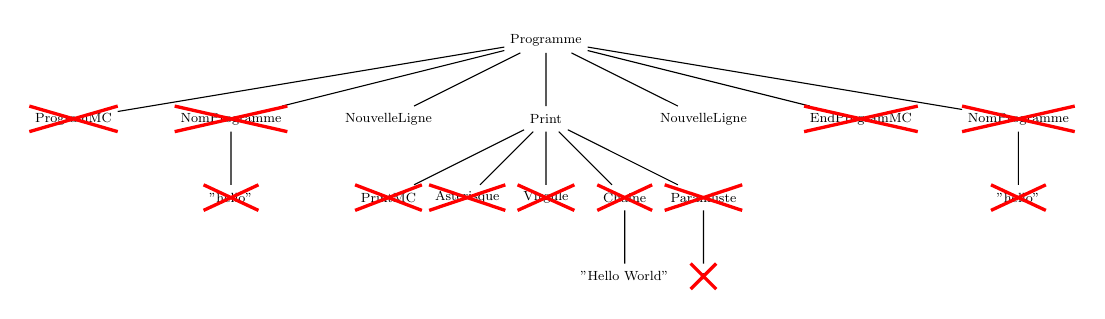
\begin{tikzpicture}
    [
        baseline=(0), 
        level/.style={sibling distance = 2cm/#1, level distance = 1cm},
        every node/.style={scale=0.6, font=\footnotesize, minimum width=15pt, minimum height=15pt}
    ]
    
    \node at (0, 0) { };
    \begin{scope}[shift={(5, 0)}]
        \node {Programme}
            child {node (0) {ProgramMC}}
            child {node (1) {NomProgramme}
                child {node (2) {"hello"}}
            }
            child {node {NouvelleLigne}}
            child {node {Print}
                child {node (3) {PrintMC}}
                child {node (4) {Asterisque}}
                child {node (5) {Virgule}}
                child {node (6) {Chaine}
                    child {node {"Hello World"}}
                }
                child{node (7) {Paramliste}
                    child {node (8) {$\varepsilon$}}
                }
            }
            child {node {NouvelleLigne}}
            child {node (9) {EndProgramMC}}
            child {node (10) {NomProgramme}
                child {node (11) {"hello"}}
            }
        ;
        \only<2>{\foreach \step in {0,1,...,11}{\drawcross{\step}}}
    \end{scope}
\end{tikzpicture}}
\end{frame}

\begin{frame}
  \begin{center}
    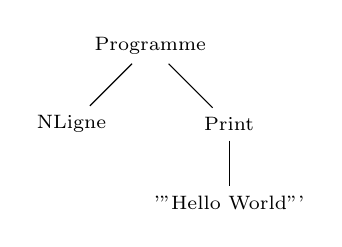
\begin{tikzpicture}

    \node[font=\scriptsize] (0) at (0, 0) {Programme};
    \node[font=\scriptsize] (1) at (-1, -1) {NLigne};
    \node[font=\scriptsize] (2) at (1, -1) {Print};
    \node[font=\scriptsize] (3) at (1, -2) {'"Hello World"'};
    
    \draw (0) -- (1);
    \draw (0) -- (2);
    \draw (2) -- (3);
\end{tikzpicture}
  \end{center}
\end{frame}
      \or
      \section{Traduction vers le langage de sortie}
\begin{frame}
  \frametitle{Traduction}

  \begin{tikzpicture}
    % frame
    \node[frame] (frame) {};
    \tikzstyle{faded}=[draw=black!20,color=black!20]
    
    \node[below=4cm of frame.west, anchor=west, box, faded] (state_1) {\scriptsize Analyse Lexicale};
    \node[right=0.5cm of state_1.east, anchor=west, box, faded] (state_2) {\scriptsize Analyse Syntaxique};
    \node[right=0.5cm of state_2.east, anchor=west, box, faded] (state_3) {\scriptsize Syntaxe Abstraite};
    \node[right=0.5cm of state_3.east, anchor=west, box] (state_4) {\scriptsize Conversion};
    \draw[->, >=latex, faded] (state_1.east) -- (state_2.west);
    \draw[->, >=latex, faded] (state_2.east) -- (state_3.west);
    \draw[->, >=latex, faded] (state_3.east) -- (state_4.west);
    \draw[dashed] (frame.south west) -- (state_4.north west);
    \draw[dashed] (frame.south east) -- (state_4.north east);

    \node(def){parcours en profondeur};
    \node[below] at (def.south) {convertion en chaîne};

  \end{tikzpicture}

\end{frame}
      \else
      \begin{frame}
        \usetikzlibrary {fit}
        \frametitle{Transpileur}
        \input{figures/transpiler_etape_\arabic{i}.tex}
      \end{frame}
    \fi
}